\documentclass[../../spr.tex]{subfiles}

\begin{document}

\newpage
\section{Implementacja}

\subsection{Opis głównych funkcjonalności aplikacji}

\begin{itemize}
  \item \textbf{Autoryzacja z wykorzystaniem OIDC} – aplikacja wykorzystuje protokół OpenID Connect (OIDC) do bezpiecznej autoryzacji i uwierzytelniania użytkowników. Dzięki temu możliwe jest logowanie przy użyciu zewnętrznych dostawców tożsamości (np. Google, Facebook), a także bezpieczne zarządzanie sesją użytkownika.

  \item \textbf{Płatności} – integracja z zewnętrznym providerem płatności  (Stripe) umożliwia użytkownikom szybkie i bezpieczne opłacanie karnetów.

  \item \textbf{Zarządzanie siłownią} – kompleksowy panel administracyjny pozwala na:
        \begin{itemize}
          \item zarządzanie karnetami (tworzenie, edycja),
          \item zarządzanie pracownikami,
          \item organizowanie sesji treningowych,
          \item monitorowanie statystyk użytkowników (liczba odbytych treningów, aktywność, postępy),
          \item obsługę zgłaszania konserwacji sal.
        \end{itemize}
\end{itemize}

\newpage
\subsection{Prezentacja zrzutów ekranu (screeny) prezentujących działanie aplikacji.}
\begin{figure}[H]
  \centering
  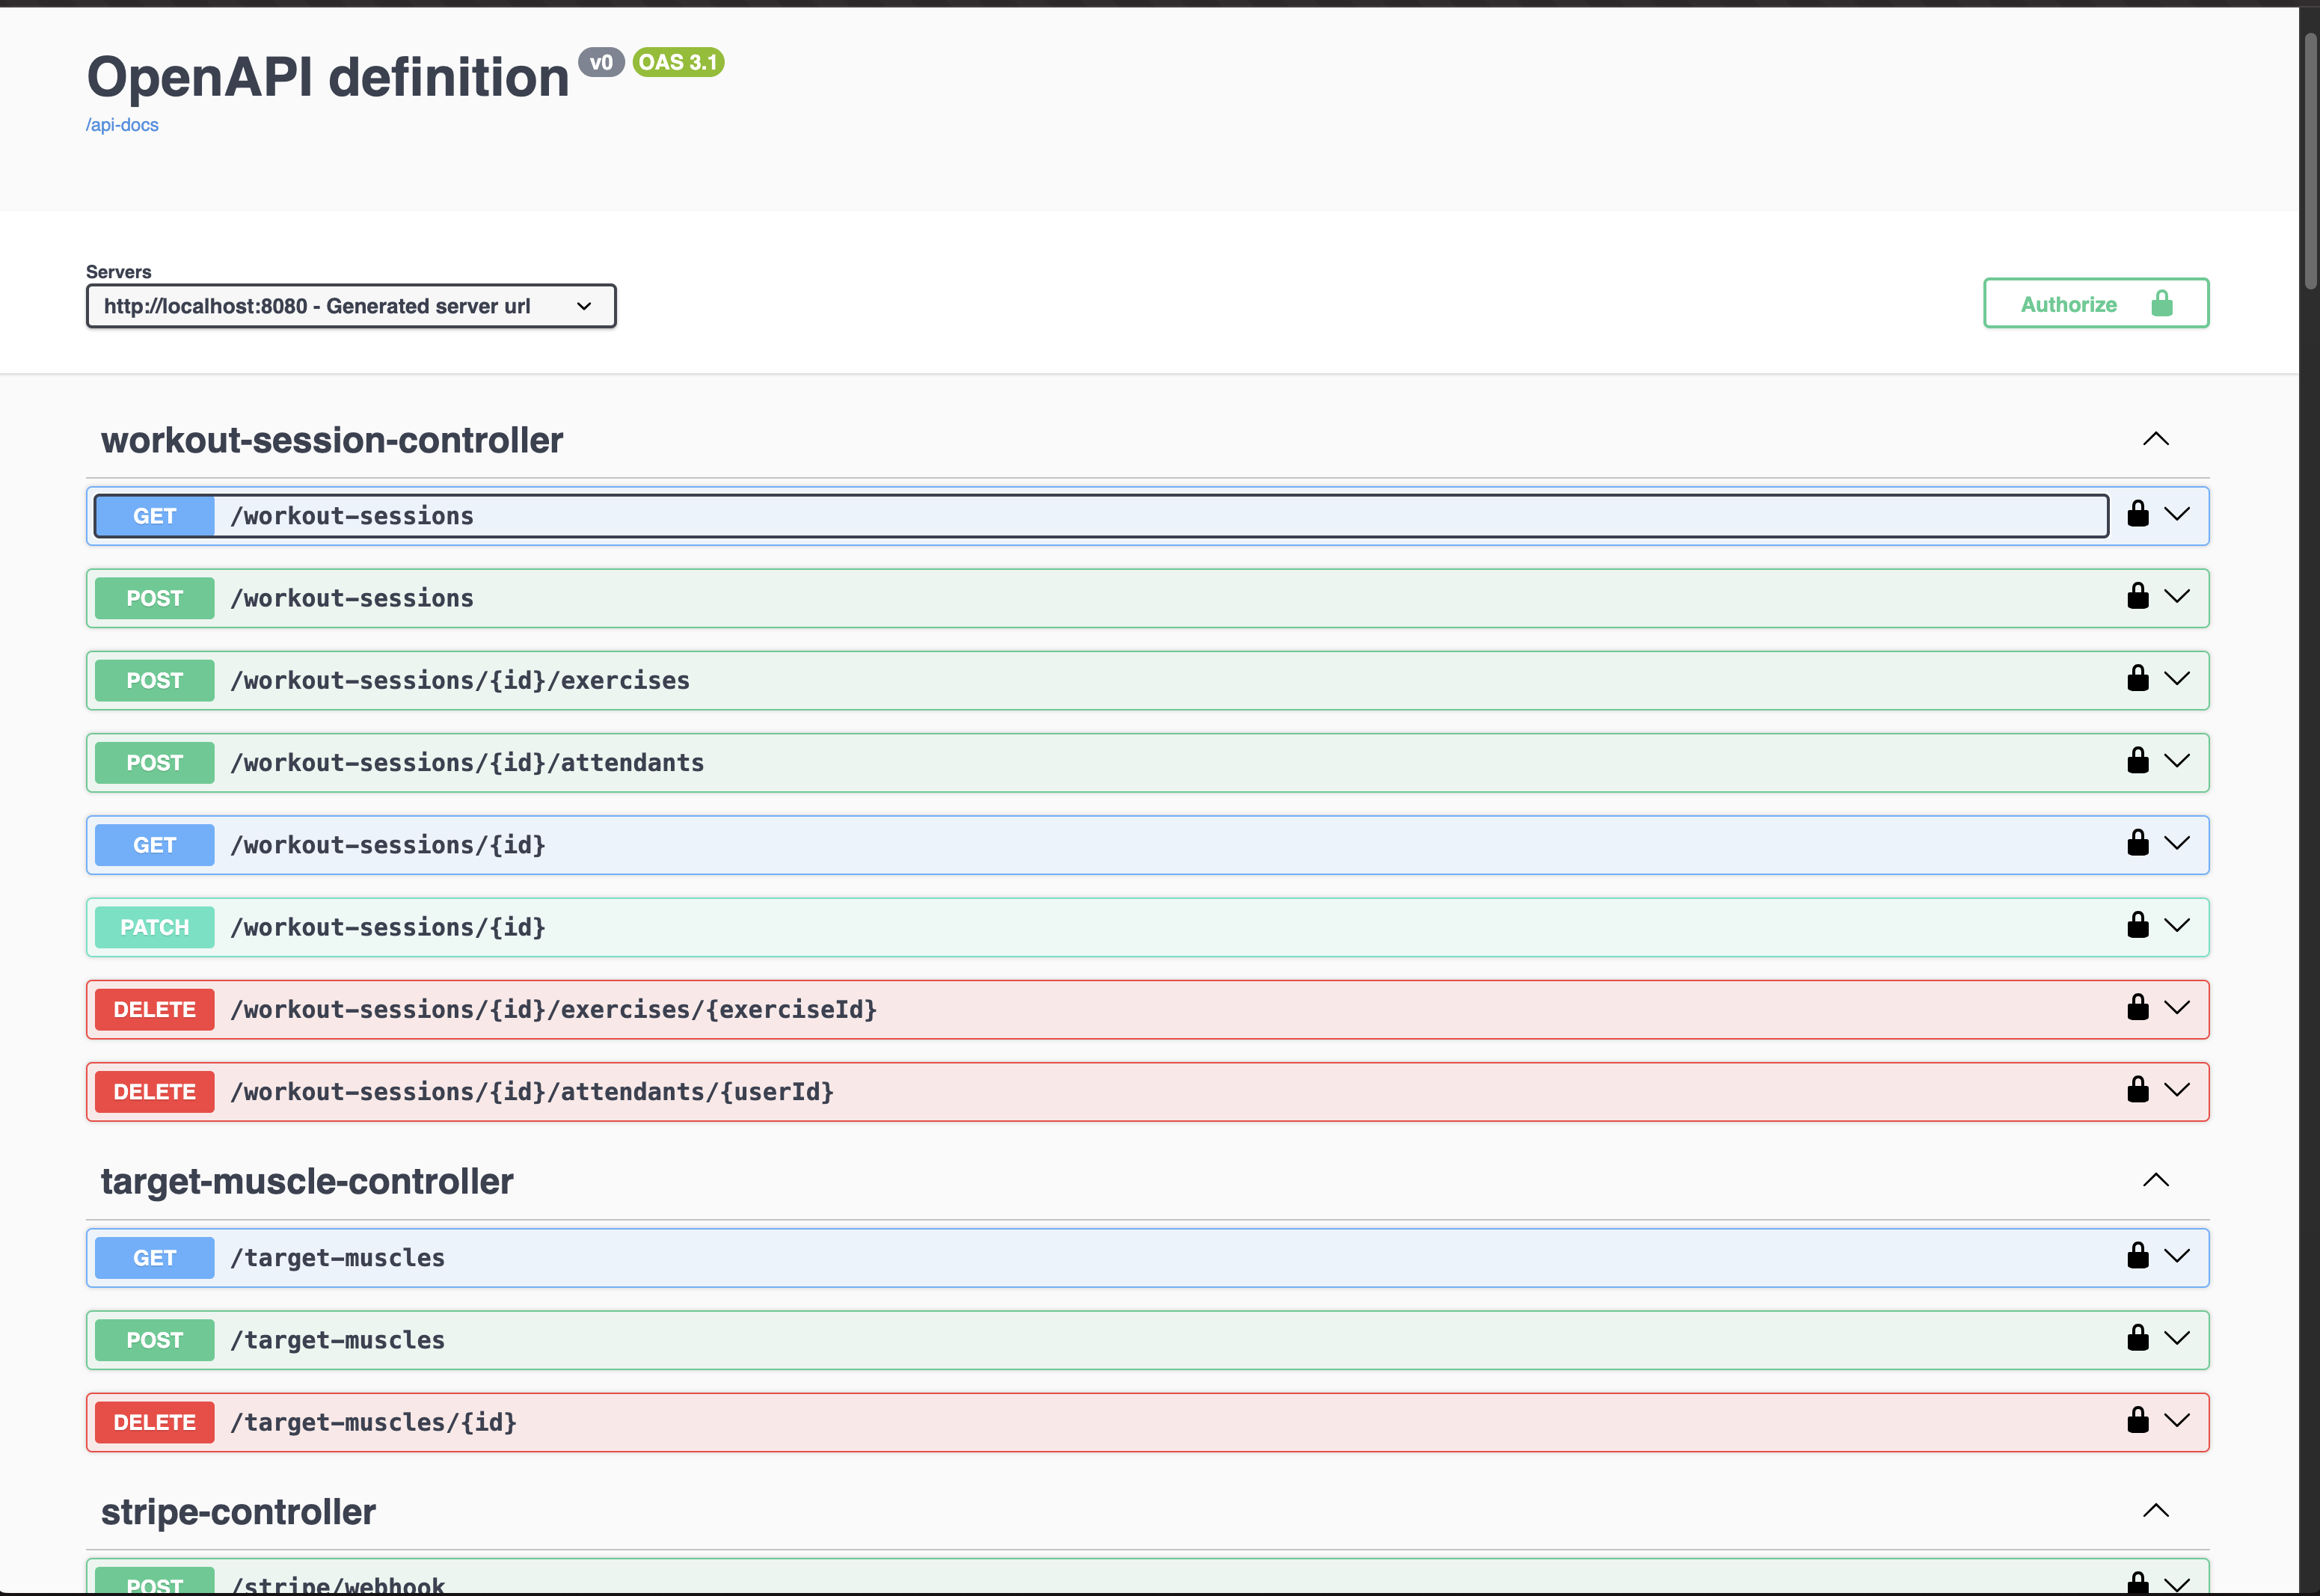
\includegraphics[width=\textwidth]{swagger.png}
  \caption{Swagger UI z dokumentacją API.}
\end{figure}

\begin{figure}
  \centering
  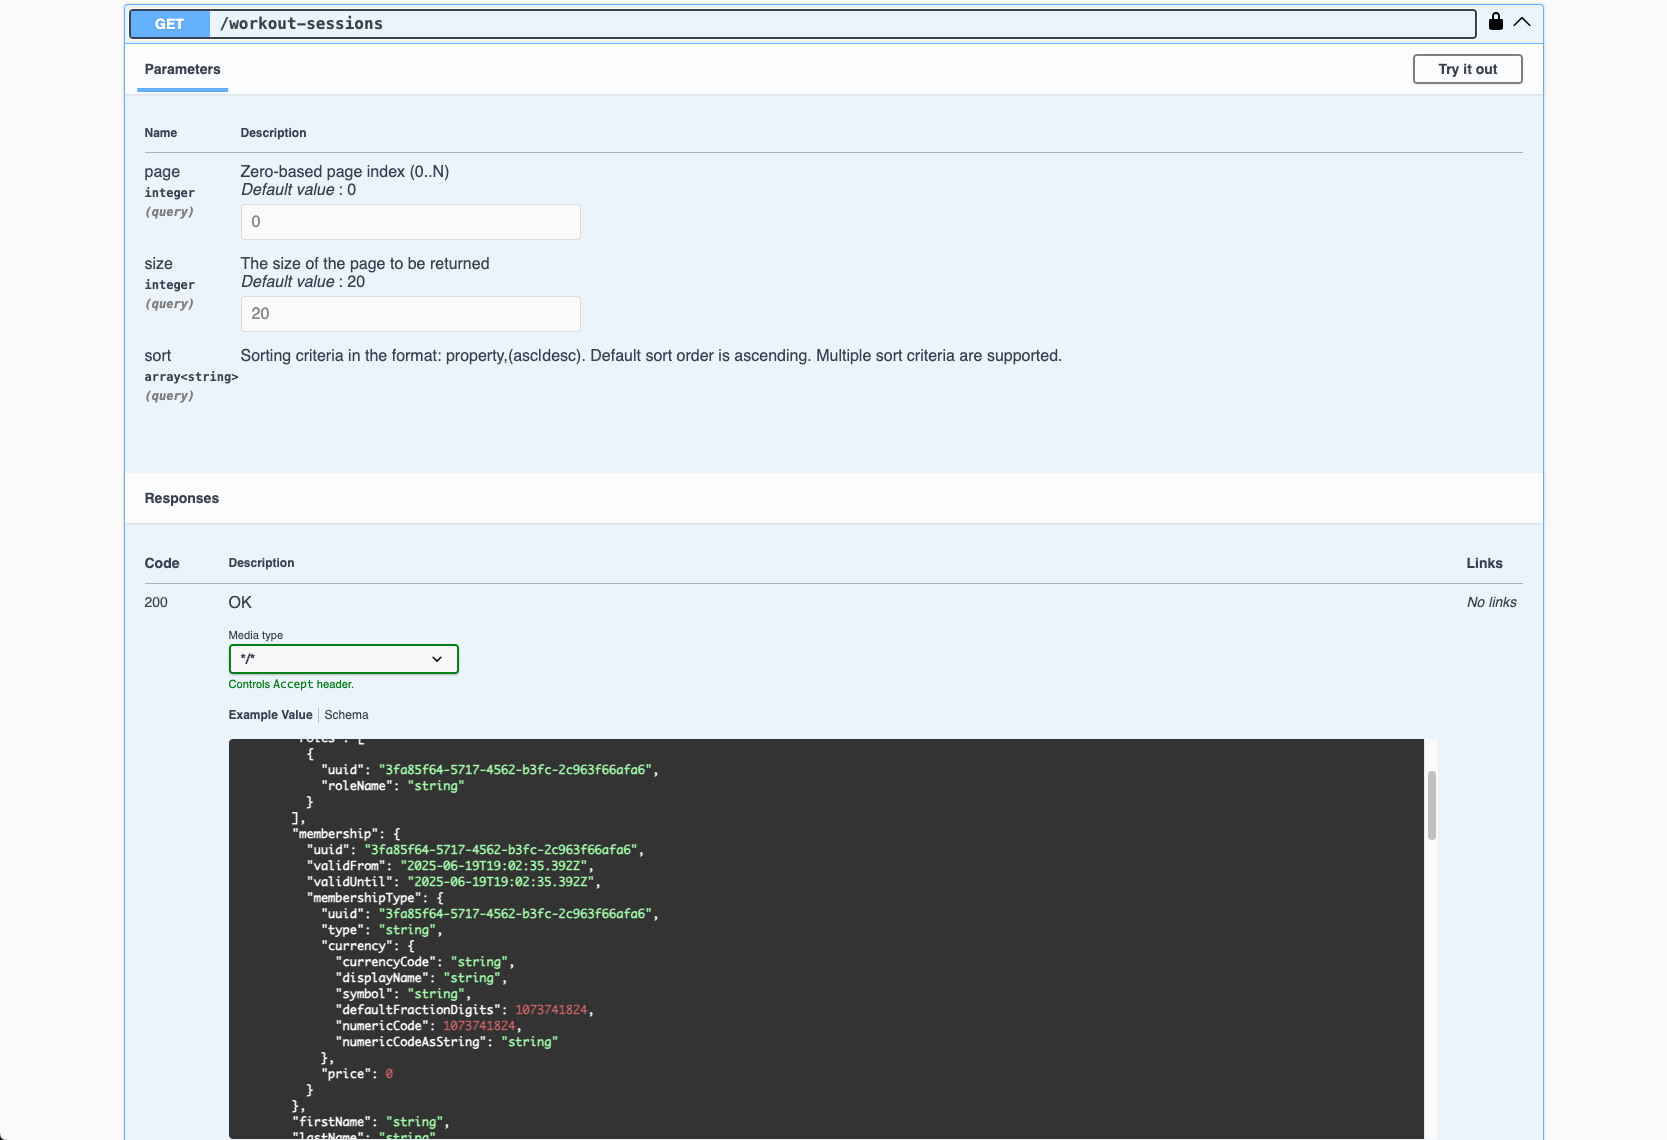
\includegraphics[width=\textwidth]{swaggerget.png}
  \caption{Swagger UI z endpointem GET.}
\end{figure}

\begin{figure}
  \centering
  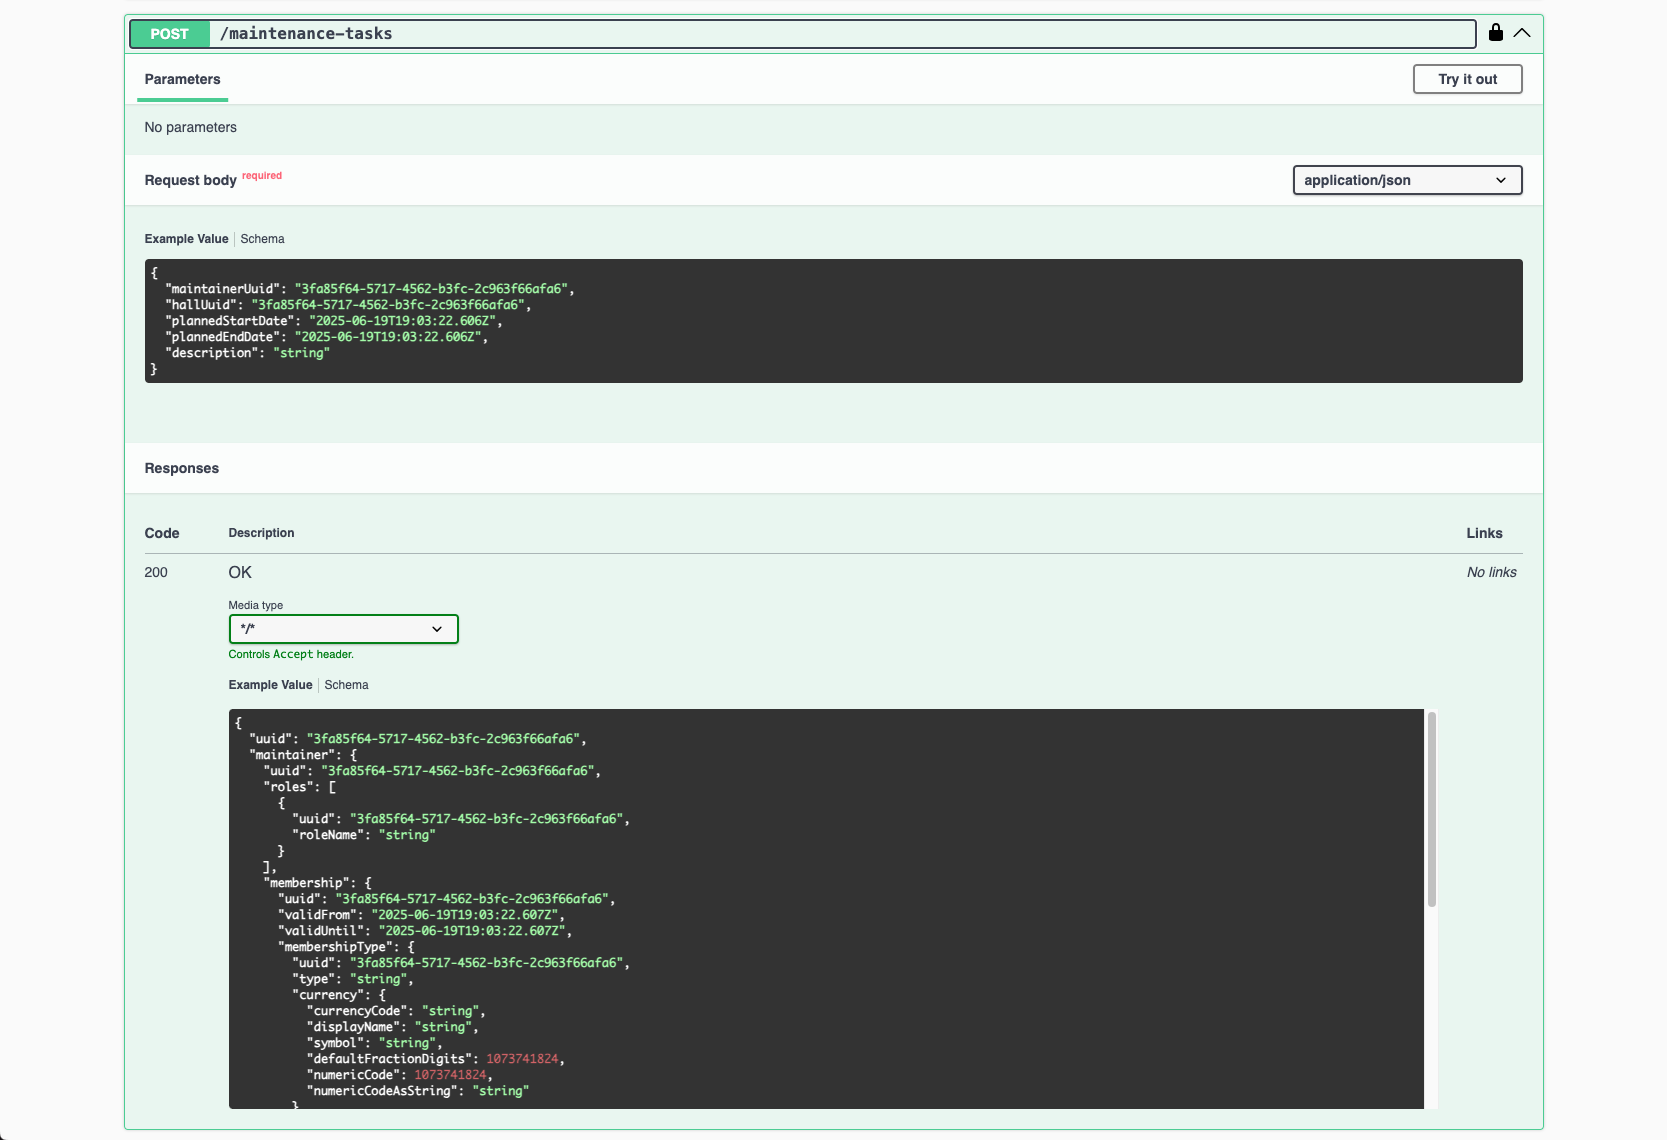
\includegraphics[width=\textwidth]{swaggerpost.png}
  \caption{Swagger UI z endpointem POST.}
\end{figure}

\begin{figure}
  \centering
  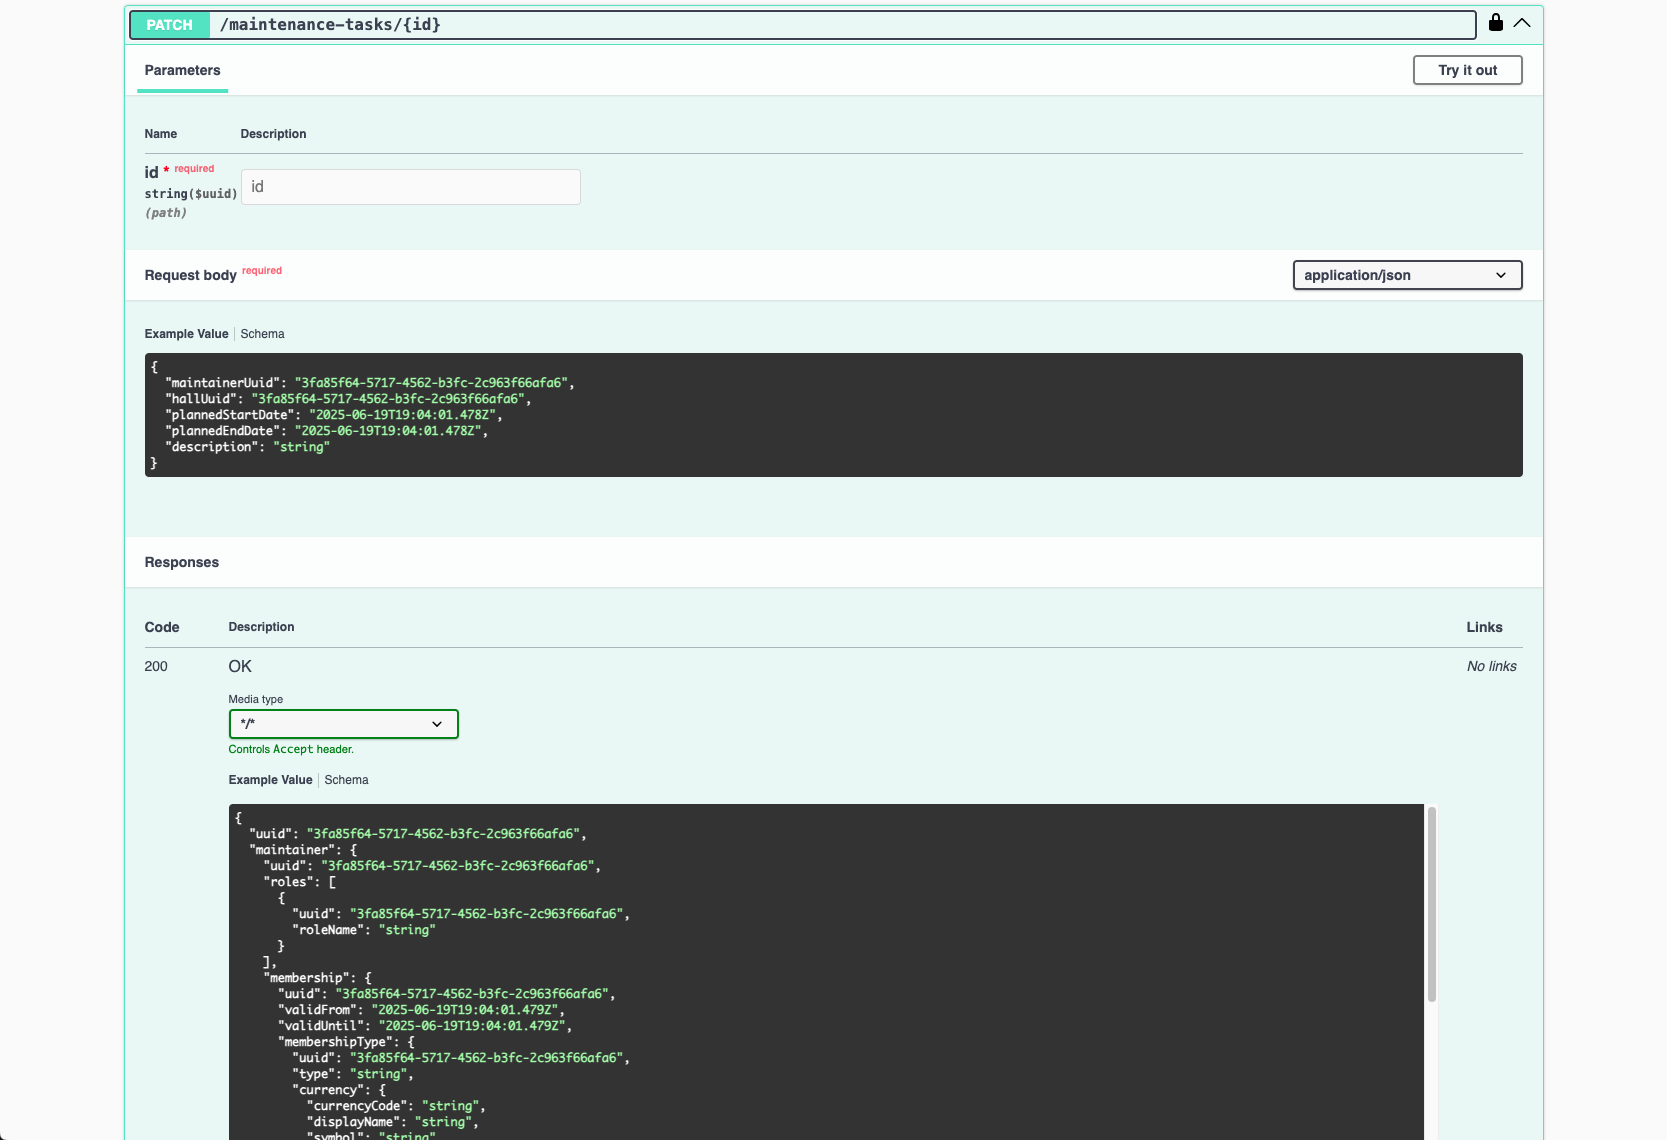
\includegraphics[width=\textwidth]{swaggerpatch.png}
  \caption{Swagger UI z endpointem PATCH.}
\end{figure}

\begin{figure}
  \centering
  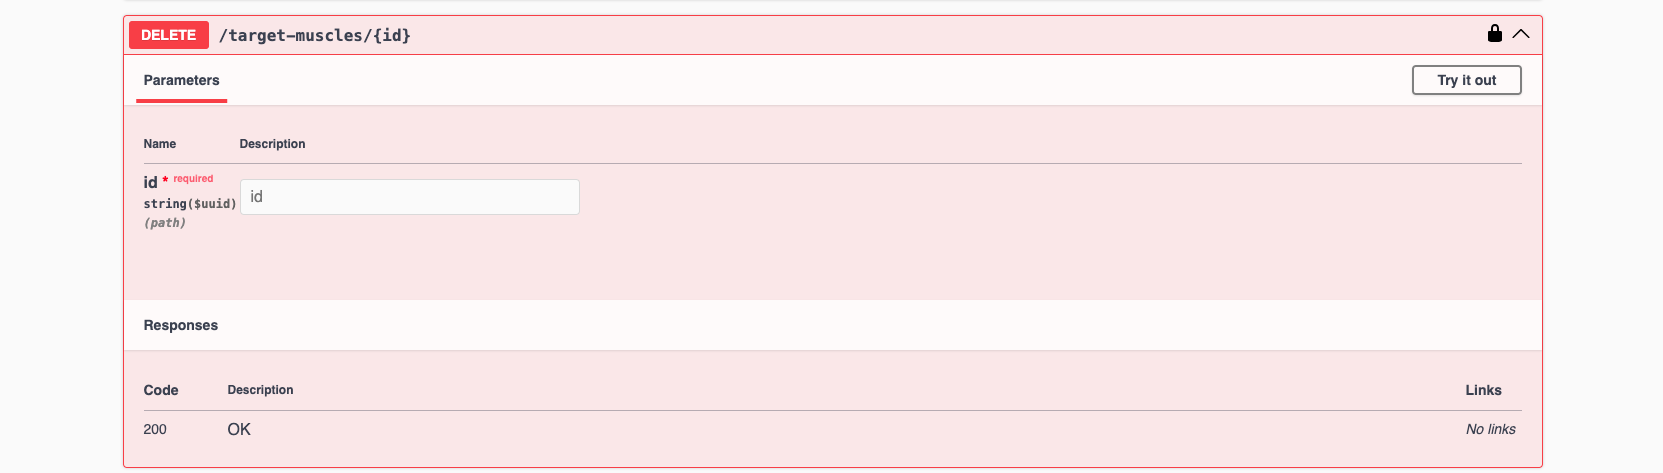
\includegraphics[width=\textwidth]{swaggerdelete.png}
  \caption{Swagger UI z endpointem DELETE.}
\end{figure}

\FloatBarrier

\subsection{Wybrane fragmenty kodu z kluczowymi funkcjonalnościami}


\subsubsection{Autoryzacja z tokena JWT}

\captionsetup{hypcap=false}
\begin{center}
  \inputminted[
    breaklines,
    fontsize=\footnotesize,
    breakanywhere,
    numbers=left
  ]{java}{./sections/implementacja/GymJwtAuthenticationConverter.java}
  \captionof{listing}{Autoryzacja z tokena JWT (OIDC).}
\end{center}


\begin{center}
  \inputminted[
    breaklines,
    fontsize=\footnotesize,
    breakanywhere,
    numbers=left
  ]{java}{./sections/implementacja/HallController.java}
  \captionof{listing}{Przykładowy kontroler obsługujący sale treningowe.}
\end{center}

\begin{center}
  \inputminted[
    breaklines,
    fontsize=\footnotesize,
    breakanywhere,
    numbers=left
  ]{java}{./sections/implementacja/HallServiceImpl.java}
  \captionof{listing}{Przykładowy serwis obsługujący sale treningowe.}
\end{center}

\begin{center}
  \inputminted[
    breaklines,
    fontsize=\footnotesize,
    breakanywhere,
    numbers=left
  ]{java}{./sections/implementacja/HallControllerTest.java}
  \captionof{listing}{Testy dotyczace sal treninigowych}
\end{center}


\end{document}